\documentclass[a4paper,11pt,svgnames,dvipsnames]{article}

\usepackage{amsmath,amssymb}
\usepackage{txfonts}

% \pi is not a variable therefore should not be italicized
\usepackage[LGR,T1]{fontenc}
\usepackage[greek,british]{babel}
\let\mathpi\pi
\renewcommand{\pi}{\text{\textrm{\greektext p}}}
% same for e
\newcommand{\e}{\mathrm{e}}

% Mimic APA7's margin requirement
\usepackage[margin=1in]{geometry}
\setlength\parindent{.5in}
\usepackage[document]{ragged2e}
\setlength{\RaggedRightParindent}{\parindent}
\usepackage{indentfirst}

% Insert PDF pages
\usepackage[final]{pdfpages}

% Insert R code
\usepackage{listings}
\usepackage{lstfiracode}
\usepackage{fontspec}
\setmonofont{Fira Code}[Contextuals=Alternate]
\lstset{
    language=R,
    columns=fullflexible,
    frame=leftline,
    % Line numbers
    numbers=left,
    numberstyle=\footnotesize\ttfamily\color{Grey},
    stepnumber=5,
    firstnumber=1,
    numberfirstline=true
    % Line breaks
    tabsize=4,
    showstringspaces=false,
    breaklines=true,
    postbreak=\mbox{\textcolor{red}{$\hookrightarrow$}\space},
    breakatwhitespace=false,
    % Fonts and tyles
    style=FiraCodeStyle,
    basicstyle=\footnotesize\ttfamily,
    stringstyle=\color{BrickRed},
    otherkeywords={0,1,2,3,4,5,6,7,8,9},
    morekeywords={TRUE,FALSE},
    deletekeywords={data,frame,length,as,character},
    keywordstyle=\color{RoyalBlue},
    commentstyle=\color{Grey},
}

\newcommand{\wrt}{with respect to }
\newcommand{\mle}[1]{\widehat{#1}_\text{MLE}}
\newcommand{\dd}[1]{\frac{\mathrm{d}}{\mathrm{d}#1}}
\newcommand{\pp}[1]{\frac{\partial}{\partial#1}}
\renewcommand{\hat}{\widehat}

\begin{document}
\RaggedRight

\section{Task Statement}

We received $n$ data points, $x_1, x_2, \ldots, x_{n}$, and were told that some of them were iid draws from an exponential distribution $\text{Exp}(\lambda)$ and some were generated from a normal distribution $\mathcal{N}(\mu, \sigma^2)$. We further learnt that smaller values were more likely to come from the exponential distribution and larger ones were more likely to come from the normal distribution. We need to decide how many (say $k$) of the $n$ data points were from the exponential (hence $n-k$ from the normal) and estimate the parameters $\lambda$, $\mu$, and $\sigma^2$.

\section{Derivation of Parameter Estimates}

We may firstly sort the data in ascending order. Next, we examine the likelihood function for this size-$n$ dataset:
\begin{equation}\label{lik}
    \mathcal{L}(\lambda, \mu, \sigma^2) = \prod_{i=1}^k \lambda \e^{-\lambda x_i} \prod_{j=k+1}^n \frac{1}{\sqrt{2\pi\sigma^2}} \e^{-\frac{\left( x_j-\mu \right)^2}{2\sigma^2}},
\end{equation}
where $k$ (more precisely the mid-way point $[k + (k+1)]/2$) is the cut-off point between the exponential and normal distributions.

The log-likelihood therefore is
\begin{equation}\label{loglik}
    \begin{aligned}
        \ell(\lambda, \mu, \sigma^2)
        & = \log\left\{ \prod_{i=1}^k \lambda \e^{-\lambda x_i} \prod_{j=k+1}^n \frac{1}{\sqrt{2\pi\sigma^2}} \e^{-\frac{\left( x_j-\mu \right)^2}{2\sigma^2}} \right\}              \\
        & = \left\{ \log\left[ \lambda^k \right] + \log\left[ \prod_{i=1}^n \e^{-\lambda x_i} \right] \right\}
        + \left\{ \log \left[ \left( 2\pi\sigma^2 \right)^{-\frac{1}{2}(n-k)} \right] + \log \left[ \prod_{j=k+1}^n \e^{-\frac{\left( x_j-\mu \right)^2}{2\sigma^2}} \right] \right\} \\
        & = k\log\lambda - \lambda\sum_{i=1}^k x_i - \frac{n-k}{2}\log\left( 2\pi\sigma^2 \right) - \frac{1}{2\sigma^2}\sum_{j=k+1}^n \left( x_j-\mu \right)^2.
    \end{aligned}
\end{equation}

We may use maximum likelihood to estimates $\lambda$, $\mu$, and $\sigma^2$.

Differentiate $\ell$ \wrt $\lambda$:
\begin{equation*}
    \frac{\partial\ell}{\partial\lambda} = \frac{k}{\lambda} - \sum_{i=1}^k x_i.
\end{equation*}
Apply first order condition:
\begin{equation}\label{foc1}
    \frac{k}{\mle{\lambda}} = \sum_{i=1}^k x_i\ \Longrightarrow\ \mle{\lambda} = \frac{k}{\sum_{i=1}^k x_i}.
\end{equation}

Differentiate $\ell$ \wrt $\mu$:
\begin{equation*}
    \begin{aligned}
        \frac{\partial\ell}{\partial\mu}
        & = -\frac{1}{2\sigma^2} \sum_{j=k+1}^n \pp{\mu} \left[ \left( x_j - \mu \right)^2 \right]
        = -\frac{1}{2\sigma^2} \sum_{j=k+1}^n \left[ 2\left( x_j - \mu \right)(-1) \right]          \\
        & = \frac{1}{\sigma^2}\sum_{j=k+1}^n \left( x_j-\mu \right)
        = \frac{1}{\sigma^2}\sum_{j=k+1}^n x_j - \frac{n-k}{\sigma^2} \mu.
    \end{aligned}
\end{equation*}
Apply first order condition:
\begin{equation}\label{foc2}
    \frac{n-k}{\sigma^2}\mle{\mu} = \frac{1}{\sigma^2}\sum_{j=k+1}^n x_j\ \Longrightarrow\ \mle{\mu} = \frac{1}{n-k}\sum_{j=k+1}^n x_j.
\end{equation}

Differentiate $\ell$ \wrt $\sigma^2$:
\begin{equation*}
    \begin{aligned}
        \frac{\partial\ell}{\partial\sigma^2}
        & = -\frac{n-k}{2}\frac{1}{2\pi\sigma^2}(2\pi)-\pp{\sigma^2} \left[ \frac{1}{2}\left( \sigma^2 \right)^{-1} \sum_{j=k+1}^n \left( x_j - \mu \right)^2 \right] \\
        & = -\frac{n-k}{2} \left( \sigma^2 \right)^{-1} - \left( -\frac{1}{2} \right) \left( \sigma^2 \right)^{-2} \sum_{j=k+1}^n \left( x_j - \mu \right)^2          \\
        & = -\frac{n-k}{2\sigma^2} + \frac{1}{2\left( \sigma^2 \right)^2} \sum_{j=k+1}^n \left( x_j-\mu \right)^2.
    \end{aligned}
\end{equation*}
Apply first order condition:
\begin{equation}\label{foc3}
    \frac{\sum_{j=k+1}^n \left( x_j - \mu \right)^2}{\left( \mle{\sigma}^2 \right)^2} = \frac{n-k}{\mle{\sigma}^2}\ \Longrightarrow\ \mle{\sigma}^2 = \frac{1}{n-k} \sum_{j=k+1}^n \left( x_j-\mu \right)^2.
\end{equation}

To summarise, the MLEs of $\lambda$, $\mu$, and $\sigma^2$ are
\begin{equation}\label{mle}
    \left\{
    \begin{aligned}
        \mle{\lambda}  & = \frac{k}{\sum_{i=1}^k x_i},                            \\
        \mle{\mu}      & = \frac{1}{n-k}\sum_{j=k+1}^n x_j,                       \\
        \mle{\sigma}^2 & = \frac{1}{n-k} \sum_{j=k+1}^n \left( x_j-\mu \right)^2.
    \end{aligned}
    \right.
\end{equation}

\section{Determine Cut-off $\boldsymbol{k}$}

Substitute (\ref{mle}) to (\ref{loglik}):
\begin{equation}\label{loglikhat}
    \begin{aligned}
        \mle{\ell}(k)
        & = k \log \left[ \frac{k}{\sum_{i=1}^k x_i} \right] - \frac{k}{\sum_{i=1}^k x_i} \sum_{i=1}^k x_i - \frac{n-k}{2} \log \left[ \frac{2\pi}{n-k} \sum_{j=k+1}^n \left( x_j - \mu \right)^2 \right] - \frac{1}{2} \frac{n-k}{\sum_{j=k+1}^n \left( x_j - \mu \right)^2} \sum_{j=k+1}^n \left( x_j - \mu \right)^2 \\
        & = -k \log \left[ \text{mean(exp data)} \right] - k - \frac{n-k}{2} \log \left[ 2\pi\times\text{var(norm data)} \right] - \frac{n-k}{2}.%\\
        % &= k \left\{ \log \left[ \frac{k}{\sum_{i=1}^k x_i} \right] - \log\e \right\}
        % - \frac{n-k}{2} \left\{ \log \left[ \frac{2\pi}{n-k} \sum_{j=k+1}^n \left( x_j - \mu \right)^2 \right] + \log\e \right\}\\
        % &= k \left\{ \log \left[ \frac{k}{\e \sum_{i=1}^k x_i} \right] \right\} - \frac{n-k}{2} \left\{ \log \left[ \frac{2\pi\e}{n-k} \sum_{j=k+1}^n \left( x_j - \frac{1}{n-k} \sum_{j=k+1}^n x_j \right)^2 \right] \right\}\\
        % &= \log \left\{ \left[ \frac{k}{\e \sum_{i=1}^k x_i} \right]^k \left[ \frac{2\pi\e}{n-k} \sum_{j=k+1}^n \left( x_j - \frac{1}{n-k} \sum_{j=k+1}^n x_j \right)^2 \right]^{-\frac{n-k}{2}} \right\},
    \end{aligned}
\end{equation}

Notice that (\ref{loglikhat}) is now a univariate function of $k$. Since $\{ k \mid k \in \mathbb{Z}, 1 \leq k \leq n-2 \}$ (we need at least the first data point to come from the exponential in order to calculate mean(exp data), and the last two data points to calculate var(norm data)), computers can perform a grid search for $\hat{k}$ that maximises $\mle{\ell}(k)$.

\section{Simulation}

Using an \textsf{R} seed 2023, we draw 50 random samples from Exp(0.8), mixing with another 950 from $\mathcal{N}(15, 2^2)$. This dataset is shown on the left panel on the next page. The right panel shows the grid search result using (\ref{loglikhat}), yielding $\hat{k} = 50$. We take the cutoff as the mid-way point between the 50th and 51st data point, which is 6.338. This data-driven cutoff sits nicely between the two distributions, agreeing with intuition.

Following (\ref{mle}), the point estimates for $\mle{\lambda}$, $\mle{\mu}$, and $\mle{\sigma}^2$ are $0.942$, $14.854$, and $3.853$ respectively, which are not too far from true values $0.8$, $15$, and $2^2$ given the limited sample size, particularly for the exponential part.

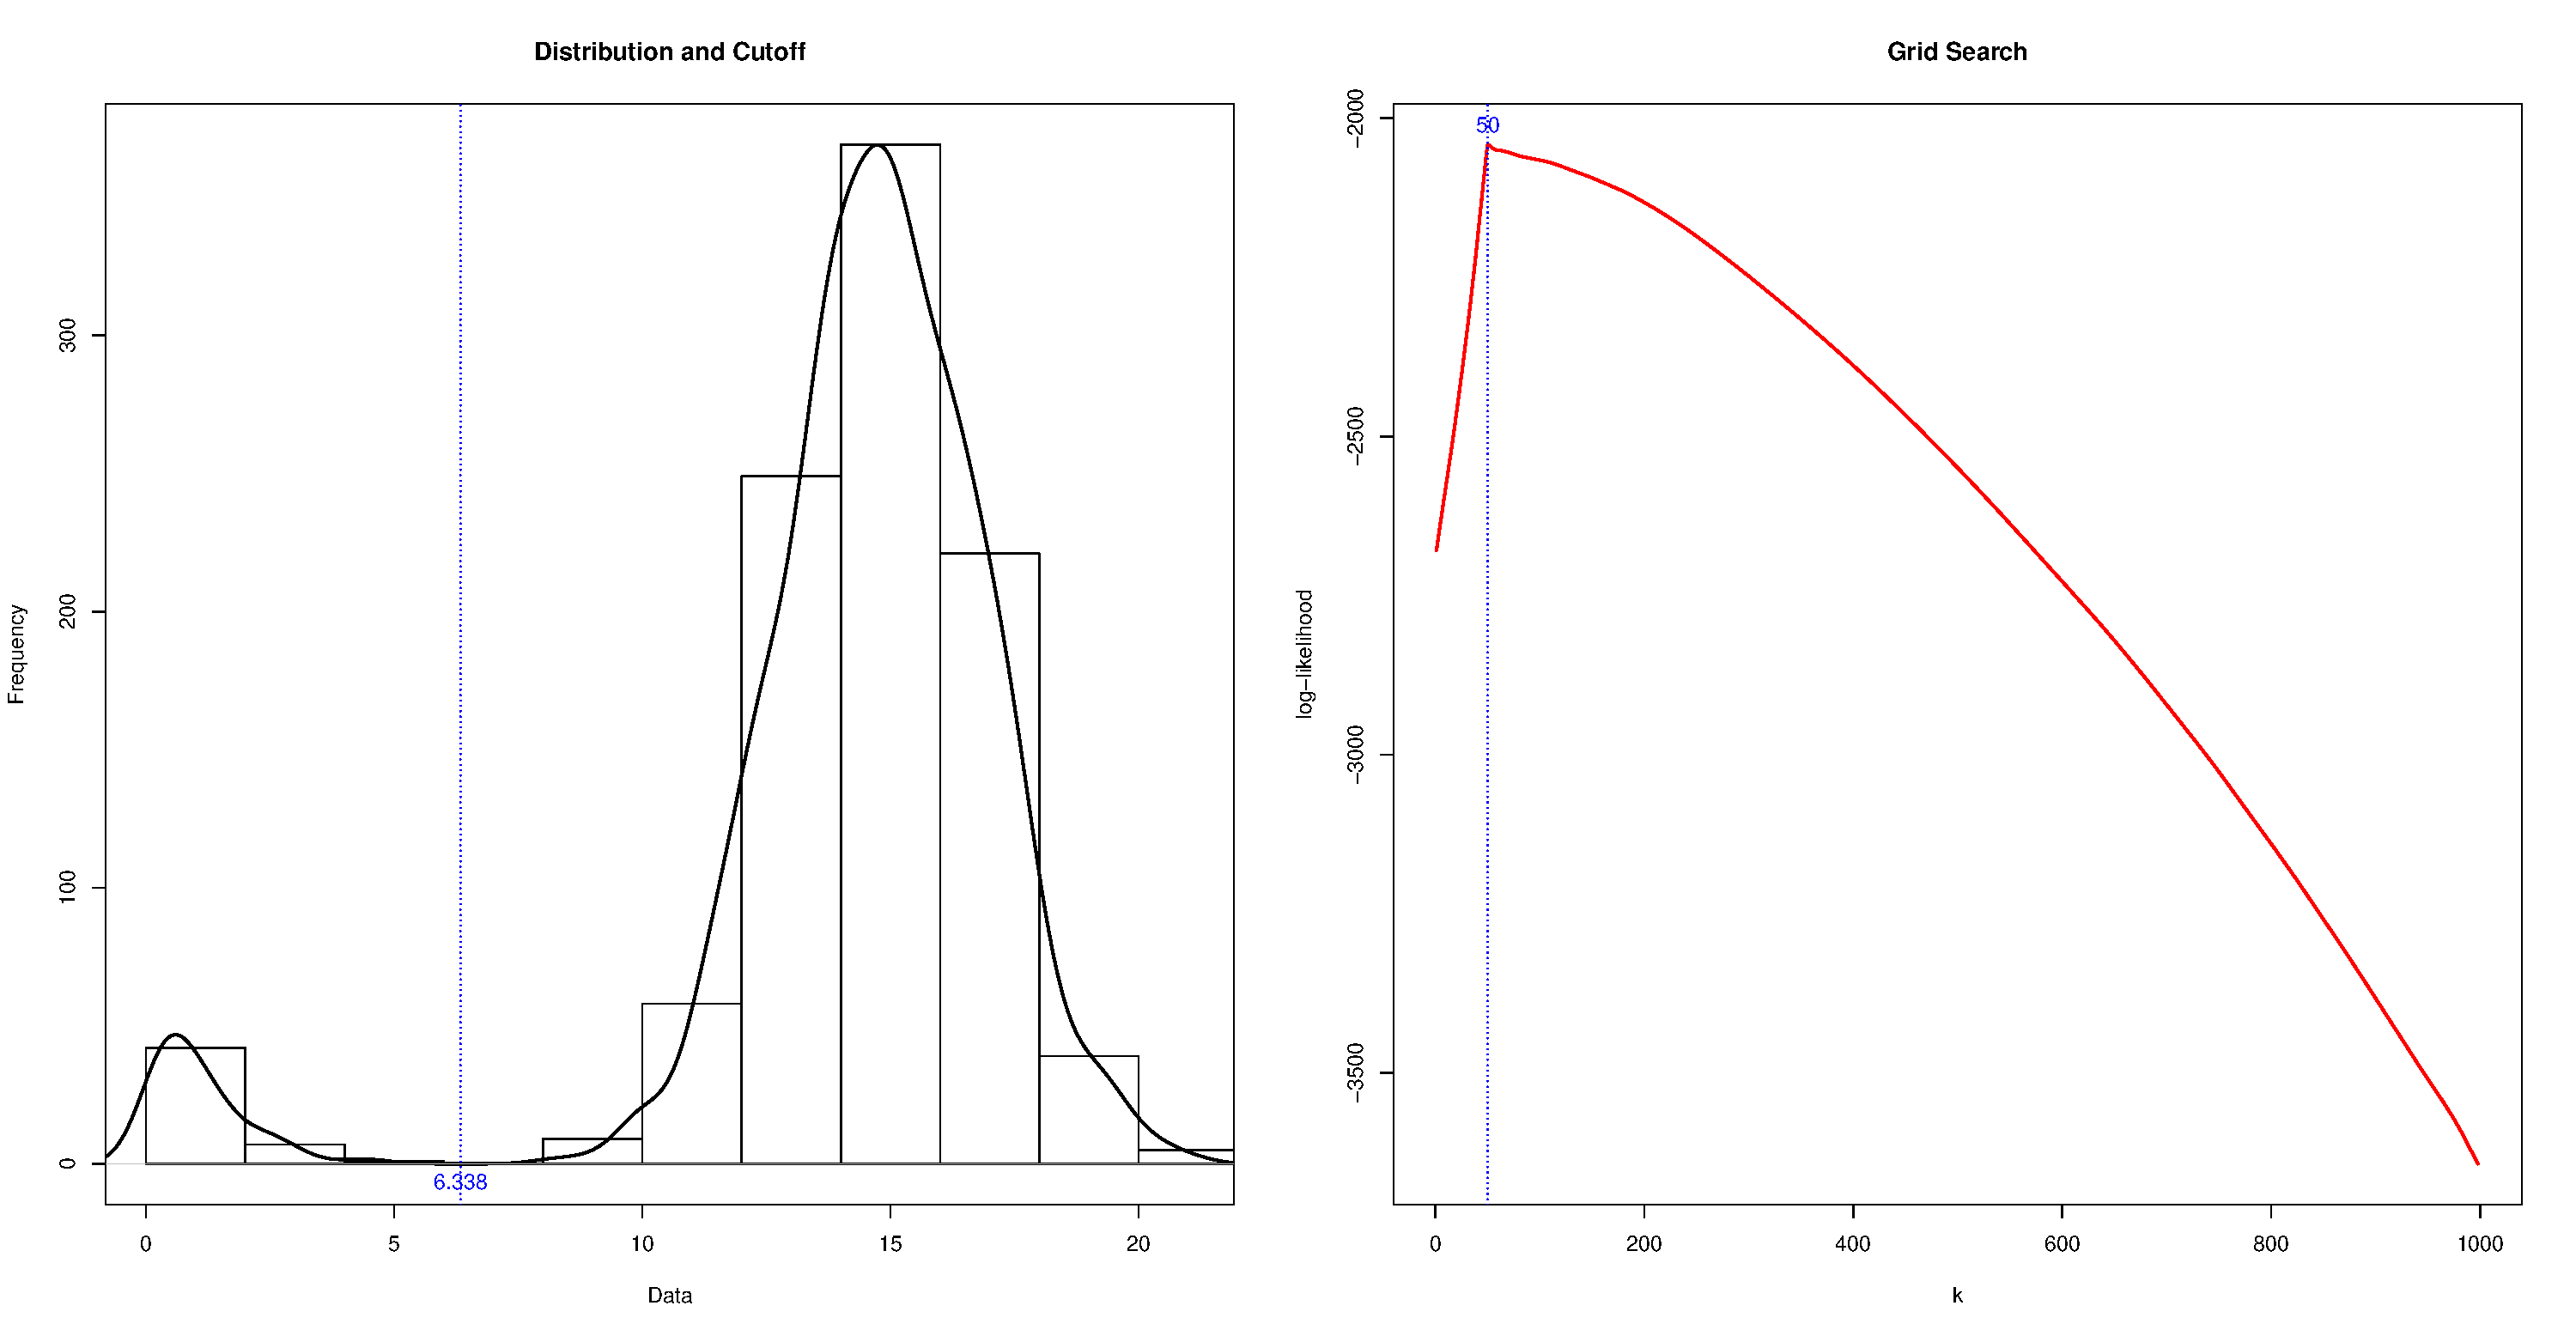
\includepdf[pages=-,angle=90,height=\textheight,pagecommand={}]{R-plot.pdf}

\section{\textsf{R} Code}

\lstinputlisting{Morten.R}

\end{document}